\documentclass{article} % For LaTeX2e
\usepackage{final_project,times}
\usepackage{pdfpages}
\usepackage{tabu}
%\documentstyle[nips12submit_09,times,art10]{article} % For LaTeX 2.09


\title{Predictive Modeling on Bank Marketing for Term Deposit}

\author{
  Menglan Jiang \\
  Department of Statistical Science\\
  Duke University\\
  Durham, NC 27708 \\
  \texttt{menglan.jiang@duke.edu} \\
  \And
  Mengrun Li \\
  Department of Statistical Science\\
  Duke University\\
  Durham, NC 27708 \\
  \texttt{mengrun.li@duke.edu} \\
  \AND
  Yaqian Cheng \\
  Department of Statistical Science\\
  Duke University\\
  Durham, NC 27708 \\
  \texttt{yaqian.cheng@duke.edu} \\
  \And
  Xinyuan Zhang \\
  Department of Electrical \& Computer Engineering\\
  Duke University\\
  Durham, NC 27708 \\
  \texttt{xy.zhang@duke.edu} \\
}


\newcommand{\fix}{\marginpar{FIX}}
\newcommand{\new}{\marginpar{NEW}}

\nipsfinalcopy

\begin{document}


\maketitle

\begin{abstract}
In this paper, we aim to research the subscription of term deposit based on clients' personal information in order to achieve optimal bank marketing strategy. Three statistical methods are employed, including the logistic regression, LASSO and SVM. SVM provides the best prediction rate while the other techniques also show great performance. LASSO helps to select significant covariates among all candidate variables.
\end{abstract}

\section{Introduction}
\label{introduction}
Bank marketing has been an emerging study in making optimal strategy to attract potential clients. It covers a wide range of businesses of banks. In bank marketing analysis, the fundamental step is to make precise prediction to differentiate potential clients from the client pool. In order to achieve this goal, various methods are applied including both quantitative and qualitative methods. \\\\
In this paper, we are particularly interested in predicting whether the client will subscribe a bank term deposit. As known to all, banks live on term deposit to proceed a series of derivative businesses. A high term deposit rate is a crucial factor to guarantee a bank's competitiveness. Hence, forecasting the decision of different clients based on the personal information stored in the internal data system becomes an important task. \\\\
Given the dataset, we have 45211 records each containing the information of a single client. The information varies from demographic information, financial status to credit history. In specific, we have 16 variables of interest, including age, maritale, education, default, balance, housing, loan, contact, day, month, duration, campaign, pdays, previous, poutcome. These are all independent variables which are considered indicators affecting whether a client will subscribe the term deposit. The dependent variable, which is a $0/1$ variable, will indicate the decision of term deposit subscription. In the following analysis, the 16 variables are extended to 42 variables in total as we create dummies for some of them.\\\\
The paper will combine quantitative and qualitative methods to make predictions. 
Three statistical methods are used in the paper, including the logistic regression, LASSO and SVM. Firstly, we carry out a logistic regression to predict the possibility of term deposit subscription of a potential client. Considering the great number of independent variables in the dataset, we research significant independent variables by LASSO and then do a logistic regression on the variables selected. Meanwhile, a classification method, SVM, is also applied to serve as a second prediction method to categorize the clients pool into two groups.  \\\\
There are several goals to be achieved in this paper. First and foremost, we aim to achieve an optimal marketing strategy to attract the potential clients. Therefore, it is essential to obtain a significant prediction on term deposit subscription based on personal data given. Secondly, in accompany with the primal task, we want to testify the performance of different statistical methods in making prediction under the scenario given here. In the end, we will tentatively explore the possibility of combining different methods to make a better prediction. In conclusion, we will make prediction of the term deposit subscriptions of clients with different personal information given via different statistical methods.

\section{Methods}
From a statistical modeling perspective, the analysis of bank marketing is a typical classification problem. Classification models, in particular binary linear classification models, aim to find a linear combination of input features or covariates to separate observed data into two groups. Here in this work we employ linear regression models and support vector machines which are widely used for classification problems. For data with a big number of variables, it is very likely that only part of them make significant contribution to the final results. So the LASSO algorithm is employed to find the variables that are most responsible to represent the data. 

\subsection{Logistic Regression}
The binary logistic model is used to estimate the probability of a binary response based on one or more predictor (or independent) variables (features). To sum up: We have a binary output variable $Y$, and we want to model the conditional probability $Pr(Y|X)$ as a function of x; any unknown parameters in the function are to be estimated by maximum likelihood. \\\\
The main idea is to model the log likelihood ratio by the function $f(x)$
\begin{equation}
f(x)=\log(\frac{P(y=1|x)}{P(y=-1|x)}).
\end{equation}
Which implies
\begin{equation}
P(y=\pm1|x)=\frac{1}{1+\exp(yf(x))}.
\end{equation}
Because logistic regression predicts probabilities, rather than just classes, we can fit it using likelihood. Given data $D$ and a class of functions $f$ the MLE is
\begin{equation}
f_{MLE}{}^{*}\colon=\arg\max_{f\in\mathcal{H}}[\prod_{i=1}^{n}\frac{1}{1+\exp(y_if(x_i))}].
\end{equation}
Typically, to find the maximum likelihood estimates we would differentiate the log likelihood with respect to the parameters, set the derivatives equal to zero, and solve.

\subsection{LASSO: Least Absolute Selection and Shrinkage Operator}
The Lasso is a shrinkage and selection method for linear regression. It minimizes the usual sum of squared errors, with a bound on the sum of the absolute values of the coefficients. It has connections to soft-thresholding of wavelet coefficients, forward stagewise regression, and boosting methods. \\\\
The idea behind the lasso procedure is to minimize
\begin{equation}
\hat{\beta}\colon=\arg\max_{\beta\in\textbf{R}^P}\frac{1}{n}\sum_{i=1}^{n}(y_i-x_i{}^T\beta)^2+\lambda\|\beta\|_1,
\end{equation}
where $\|\beta\|_1=\sum_{j=1}^{p}|\beta_j|$. \\\\
The solution $\hat{\beta}_{LASSO}=\hat{\beta}_{OLS}$ for $\lambda=0$, and the solution $\hat{\beta}_{LASSO}=0$ for $\lambda=\infty$. For the lasso with regularization parameter $\lambda$, the regression coefficient $\beta$ is a $p$-dimensional vector. The idea behind the regularization path is to select how many variables are responsible to represent the data. Compared with the ridge model, it is easier to interpret a regularization parameter in the lasso model since many of its coefficients are set to zero and the changes are fast for large $\lambda$ value.

\subsection{Support Vector Mechine}
In machine learning, support vector machines are supervised learning models with associated learning algorithms that analyze data and recognize patterns, used for classification and regression analysis. Given a set of training examples, each marked for belonging to one of two categories, a support vector machine constructs a hyperplane or set of hyperplanes in a high-dimensional space. Intuitively, a good separation is achieved by the hyperplane that has the largest distance to the nearest training-data point of any class (so-called functional margin).
\begin{figure}[h]
	\begin{center}
		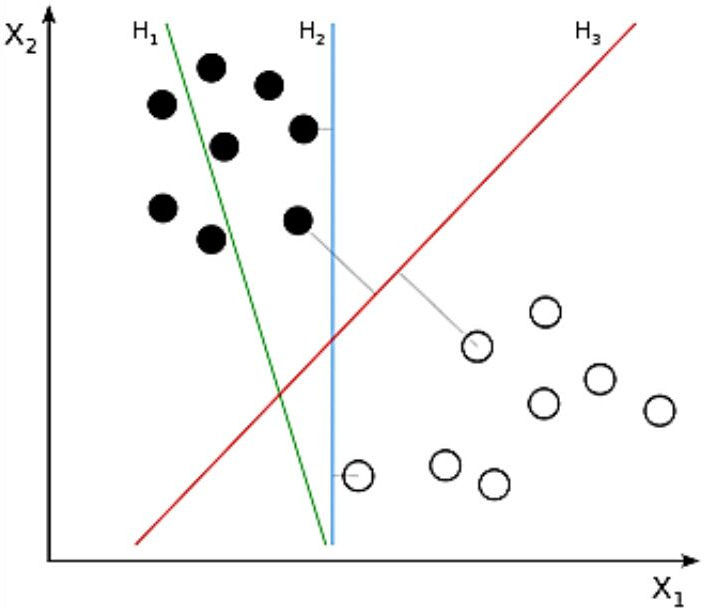
\includegraphics[scale = 0.5]{svm.png}
	\end{center}
	\caption{Support Vector Machine}
\end{figure}
In this figure, $H_1$ does not separate the classes. $H_2$ does, but only with a small margin. $H_3$ is the optimal hyperplane since it separates them with the maximum margin.


\section{Results}
\label{results}

In this section, first we are going to look at the coefficient estimates for logistic regression model and LASSO logistic regression model and find those significant variables in our models. Then, we will campare the prediction accuracy and mean squared prediction errors among those three models. 

\subsection{Logistic Regression}

We start from a simple logistic regression that is easy to work with. Coefficient estimates for logistic regression model are given in Table 5. We are looking for factors that strongly affect clients' decision of making term deposits. If we choose significance level $\alpha=0.05$, there are 33 variables out of 42 variables that are statistically significant. In this model, variables age, pdays, previous and default are unsignificant. Some dummy variables for job, marital, month and poutcome are unsignificant too. For example, variable maritalsingle is not significant. That means whether a client is single or divorced will not affect his or her probability of making term deposit. It also makes sense that many factors such as housing, loan and campaign have great effects on clients' decision in making term deposits.\\\\
Comparison between logistic regression prediction results and actual results is given in Table 1. From the result, we can tell that the prediction accuracy is 90.184\% which measures the in-sample performance of our model. Besides, we also care about the out-of-sample performance of our model. We use 10-fold cross validation to estimate prediction error and get MSE=0.071 for the logistic regressiom model.
\begin{table}[ht]
\caption{comparison between logistic regression prediction results and actual results}
\centering
\begin{tabular}{rrr}
  \hline
 & 0 & 1 \\ 
  \hline
no & 38940 & 982 \\ 
  yes & 3456 & 1833 \\ 
   \hline
\end{tabular}
\end{table}

\subsection{LASSO Logistic Regression}
\begin{figure}[h]
\begin{center}
   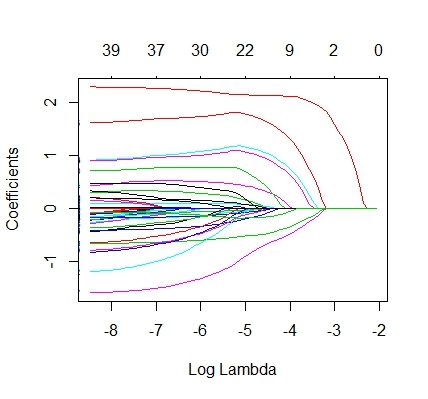
\includegraphics[scale = 0.5]{lassotraceplot.jpg}
\end{center}
\caption{lasso coefficient trace plot}
\end{figure}

From the trace plot above, we can see that when log $\lambda$ becomes larger and larger, more and more coefficients will be shrinkaged to 0.\\\\
LASSO logistic regression can do covariates selection because of using l1 penalty to shrinkage the coefficients to zero. Checking non-zero coefficients of the results, we can see that except for the intercept, there are 27 out of 42 non-zero coefficients. That means those 27 covariates are significant and contribute more to our model than those with zero coefficients. From Table 6, which is located in appendix, we can see that in job perspective, people who are students or have already retired are more likely to deposit money. That makes sense. Since retired people are usually old people, so that they need backup in case they have disease. Students who may not use their parents' money also need to deposit money to pay tuition fee. Besides, the results show that the coefficients of people who have housing loan or personal loan are significant and negative, which means they tend not to deposit. It also makes sense, because they may not have enough money to deposit after they repay the loans. In addition, successful poutcome has significant coefficient. Poutcome represents outcome of the previous marketing campaign, so that successful poutcome means the customer was attracted and deposited during the previous campaign. Therefore, in the new campaign, it is more likely for him/her to continue deposit in the same bank.
\begin{table}[ht]
\caption{comparison between LASSO prediction results and real results}
\centering
\begin{tabular}{rrr}
  \hline
 & 0 & 1 \\ 
  \hline
no & 39085 & 837 \\ 
  yes & 3612 & 1677 \\ 
   \hline
\end{tabular}
\end{table}
From the table below, we can see that the number of true positive prediction is 1677, the number of true negative prediction is 39085, the number of false negative prediction is 3612 and it of false positive is 837. The prediction rate is 90.159\%. We also calculate mean square error of this model, which is 0.142.

\subsection{Support Vector Machine}
From the table below, we can see that the number of true positive prediction is 2159, the number of true negative prediction is 39304. The prediction rate is 91.71\%. So SVM has the highest prediction accuracy among those three models. However, SVM regression is more computationally expensive compared with the first two models especially when you want to apply cross validation to estimate the mean square error of the model.
\begin{table}[ht]
\caption{comparison between SVM prediction results and actual results}
\centering
\begin{tabular}{rrr}
  \hline
 & 0 & 1 \\ 
  \hline
no & 39304 & 618 \\ 
  yes & 3130 & 2159 \\ 
   \hline
\end{tabular}
\end{table}


\section{Conclusions}
From the results above, we can conclude that the SVM presents the best estimation for whether making the term deposit based on the personal information. The LASSO and Logistic also obtain good estimations with relatively less precise results, but have better interpretation. In logistic regression, we find 33 significant variables out of 42 candidates. In LASSO, we find out that among 42 candidate variables, approximately 27 of them make significant contribution to the decision. \\\\
Our three models present good predictions. Therefore, different methods can be employed based on the purpose of the analysis. In general, we aim to increase the proportion of clients that make term deposits. As a result, we can reach out to the most valuable clients based on the predictions made, and come up with a series of corresponding marketing strategy to make the subscription of term deposit more attractive to those clients.



\subsubsection*{References}
\small{
[1] Moro et al., (2014) S. Moro, P. Cortez and P. Rita. A Data-Driven Approach to Predict the Success of Bank Telemarketing. {\it Decision Support Systems}, Elsevier, 62:22-31, June 2014.

[2] Sayan Mukherjee. LASSO: Least Absolute Selection and Shrinkage Operator. {\it Probabilistic Machine Learning}.

[3] https://upload.wikimedia.org/wikipedia/commons/thumb/b/b5/Svm\_separating\_hyperplanes\_%28SVG%29.svg/512px-Svm\_separating\_hyperplanes\_%28SVG%29.svg.png
}

\newpage

\section{Appendix}
\subsection{Data Description}

\begin{table}[h]
\caption{description of bank dataset} 
\begin{tabu} to \hsize {|X[0.8,c]|X[2,c]|X[10,l]|}
\hline
Index&Variable&Description\\ \hline
1&age&(numeric)\\ \hline
2&job&type of job (categorical: admin., blue-collar, entrepreneur, housemaid, management, retired, self-employed, services, student, technician, unemployed , unknown)\\ \hline
3&marital&marital status (categorical: divorced, married, single, unknown; note: divorced means divorced or widowed)\\ \hline
4&education&(categorical: basic.4y, basic.6y, basic.9y, high.school, illiterate, professional.course, university.degree, unknown)\\ \hline
5&default&has credit in default? (categorical: no, yes, unknown)\\ \hline
6&balance&number of balance. (numeric)\\ \hline
7&housing&has housing loan? (categorical: no, yes, unknown)\\ \hline
8&loan&has personal loan? (categorical: no, yes, unknown)\\ \hline
9&contact&contact communication type (categorical: cellular, telephone)\\ \hline
10&month& last contact month of year (categorical: jan, feb, mar,..., nov, dec)\\ \hline
11&day of week&last contact day of the week (categorical: mon, tue, wed, thu, fri)\\ \hline
12&duration&last contact duration, in seconds (numeric).\\ \hline
13&campaign&number of contacts performed during this campaign and for this client (numeric, includes last contact)\\ \hline
14&pdays& number of days that passed by after the client was last contacted from a previous campaign (numeric; 999 means client was not previously contacted)\\ \hline
15&previous& number of contacts performed before this campaign and for this client (numeric)\\ \hline
16&poutcome& outcome of the previous marketing campaign (categorical: failure, nonexistent, success)\\ \hline
17&y&has the client subscribed a term deposit? (binary: yes, no)\\
\hline
\end{tabu}
\end{table}
\newpage
\subsection{Coefficient Estimates}
\begin{table}[h]
\caption{coefficient estimates for logistic regression model} 
\centering
{\small
\begin{tabular}{rrrrr}
  \hline
 & Estimate & Std. Error & z value & Pr($>$$|$z$|$) \\ 
  \hline
(Intercept) & -2.536 & 0.184 & -13.803 & 0.000 \\ 
  bank.age & 0.000 & 0.002 & 0.051 & 0.959 \\ 
  bank.balance & 0.000 & 0.000 & 2.493 & 0.013 \\ 
  bank.duration & 0.004 & 0.000 & 64.986 & 0.000 \\ 
  bank.campaign & -0.091 & 0.010 & -8.955 & 0.000 \\ 
  bank.pdays & -0.000 & 0.000 & -0.335 & 0.737 \\ 
  bank.previous & 0.010 & 0.007 & 1.561 & 0.118 \\ 
  jobblue.collar & -0.310 & 0.073 & -4.264 & 0.000 \\ 
  jobentrepreneur & -0.357 & 0.126 & -2.844 & 0.004 \\ 
  jobhousemaid & -0.504 & 0.136 & -3.693 & 0.000 \\ 
  jobmanagement & -0.165 & 0.073 & -2.255 & 0.024 \\ 
  jobretired & 0.252 & 0.097 & 2.596 & 0.009 \\ 
  jobself.employed & -0.298 & 0.112 & -2.664 & 0.008 \\ 
  jobservices & -0.224 & 0.084 & -2.662 & 0.008 \\ 
  jobstudent & 0.382 & 0.109 & 3.505 & 0.000 \\ 
  jobtechnician & -0.176 & 0.069 & -2.554 & 0.011 \\ 
  jobunemployed & -0.177 & 0.112 & -1.583 & 0.113 \\ 
  jobunknown & -0.313 & 0.233 & -1.342 & 0.180 \\ 
  maritalmarried & -0.179 & 0.059 & -3.046 & 0.002 \\ 
  maritalsingle & 0.092 & 0.067 & 1.375 & 0.169 \\ 
  educationsecondary & 0.184 & 0.065 & 2.833 & 0.005 \\ 
  educationtertiary & 0.379 & 0.075 & 5.031 & 0.000 \\ 
  educationunknown & 0.250 & 0.104 & 2.411 & 0.016 \\ 
  defaultyes & -0.017 & 0.163 & -0.102 & 0.918 \\ 
  housingyes & -0.675 & 0.044 & -15.395 & 0.000 \\ 
  loanyes & -0.425 & 0.060 & -7.091 & 0.000 \\ 
  contacttelephone & -0.163 & 0.075 & -2.173 & 0.030 \\ 
  contactunknown & -1.623 & 0.073 & -22.184 & 0.000 \\ 
  day & 0.010 & 0.002 & 3.993 & 0.000 \\ 
  monthaug & -0.694 & 0.078 & -8.842 & 0.000 \\ 
  monthdec & 0.691 & 0.177 & 3.912 & 0.000 \\ 
  monthfeb & -0.147 & 0.089 & -1.648 & 0.099 \\ 
  monthjan & -1.262 & 0.122 & -10.367 & 0.000 \\ 
  monthjul & -0.831 & 0.077 & -10.733 & 0.000 \\ 
  monthjun & 0.454 & 0.094 & 4.843 & 0.000 \\ 
  monthmar & 1.590 & 0.120 & 13.265 & 0.000 \\ 
  monthmay & -0.399 & 0.072 & -5.521 & 0.000 \\ 
  monthnov & -0.873 & 0.084 & -10.347 & 0.000 \\ 
  monthoct & 0.881 & 0.108 & 8.159 & 0.000 \\ 
  monthsep & 0.874 & 0.119 & 7.314 & 0.000 \\ 
  poutcomeother & 0.203 & 0.090 & 2.265 & 0.024 \\ 
  poutcomesuccess & 2.291 & 0.082 & 27.821 & 0.000 \\ 
  poutcomeunknown & -0.092 & 0.093 & -0.982 & 0.326 \\ 
   \hline
\end{tabular}
}
\end{table}
\begin{table}[t]
\caption{coefficient estimates for LASSO logistic regression model} 
\centering
{\small
\begin{tabular}{rr}
  \hline
 & estimate \\ 
  \hline
(Intercept) & -2.688 \\ 
  bank.age &  \\ 
  bank.balance & 0.000 \\ 
  bank.duration & 0.004 \\ 
  bank.campaign & -0.051 \\ 
  bank.pdays &  \\ 
  bank.previous & 0.001 \\ 
  jobblue.collar & -0.098 \\ 
  jobentrepreneur &  \\ 
  jobhousemaid & -0.029 \\ 
  jobmanagement &  \\ 
  jobretired & 0.243 \\ 
  jobself.employed &  \\ 
  jobservices &  \\ 
  jobstudent & 0.480 \\ 
  jobtechnician &  \\ 
  jobunemployed &  \\ 
  jobunknown &  \\ 
  maritalmarried & -0.119 \\ 
  maritalsingle & 0.088 \\ 
  educationsecondary &  \\ 
  educationtertiary & 0.125 \\ 
  educationunknown &  \\ 
  defaultyes &  \\ 
  housingyes & -0.572 \\ 
  loanyes & -0.285 \\ 
  contacttelephone &  \\ 
  contactunknown & -1.173 \\ 
  day &  \\ 
  monthaug & -0.185 \\ 
  monthdec & 0.762 \\ 
  monthfeb &  \\ 
  monthjan & -0.402 \\ 
  monthjul & -0.320 \\ 
  monthjun & 0.337 \\ 
  monthmar & 1.772 \\ 
  monthmay & -0.066 \\ 
  monthnov & -0.273 \\ 
  monthoct & 1.128 \\ 
  monthsep & 1.046 \\ 
  poutcomeother & 0.031 \\ 
  poutcomesuccess & 2.170 \\ 
  poutcomeunknown & -0.163 \\ 
   \hline
\end{tabular}
}
\end{table}
\end{document}
